\documentclass[a4paper, openany]{book}
\usepackage[T1]{fontenc}%per rappresentare i font italiani, come le lettere accentate, con la giusta spaziatura
\usepackage[utf8]{inputenc}%per poter inserire nel testo .tex i caratteri unicode8
\usepackage[italian]{babel}%per poter effettuare la giusta sillabazione della lingua italiana
\usepackage{classicthesis}%necessario per usare lo stile arsclassica
\usepackage{arsclassica}%per poter usare lo stile arsclassica usato nell'Arte di imparare il Latex
\usepackage{amsmath}%per poter rappresentare ed utilizzare al meglio gli ambienti e le formule matematiche
\usepackage{amssymb}%per rappresentare alcuni simboli particolari matematici
\usepackage{amsthm}%per definire e poter effettuare le dimostrazioni matematiche
\usepackage{amsfonts}%per poter avere i font matematici
\usepackage{amstext}%per avere una gestione del testo nell'ambiente matematico
\usepackage{booktabs}%per la corretta gestione delle tabelle
\usepackage{microtype}%per effettuare un aggiustamento della spaziatura tra caratteri e del font
\usepackage{clrscode3e}%per effettuare lo pseudocodice nello stile del libro CLRS
\usepackage{graphicx}
\usepackage[backend=biber,
style=alphabetic,
sorting=ynt
]{biblatex}
\addbibresource{bibliography.bib}

\theoremstyle{definition}%per avere lo stile tondo quando uso un ambiente definito da newtheorem
\newtheorem*{defi}{Def}%Definizione per avere la gestione delle definizioni
\newtheorem{prop}{Prop}[chapter]
\newtheorem{thm}{Thm}[chapter]
\newtheorem{esempio}{Esempio}
\newcommand{\numberset}{\mathbb}
\newcommand{\N}{\numberset{N}}
\newcommand{\deriv}{\Rightarrow}

\begin{document}
    \title{Computational Math notes}
    \author{Marco Natali}
    \date{}
    \maketitle 
  
    \tableofcontents
    \listoffigures

    \chapter{Introduction}
This course will provide an introduction to AI techniques and approach analyzed nowadays and to understand
the current state of art we have to provide an Timeline to see progress and discover done during the time,
so in figure \ref{img:timeline} we will see all important events related with AI.

\begin{figure}
    \caption{AI Timeline evolution}
    \label{img:timeline}
    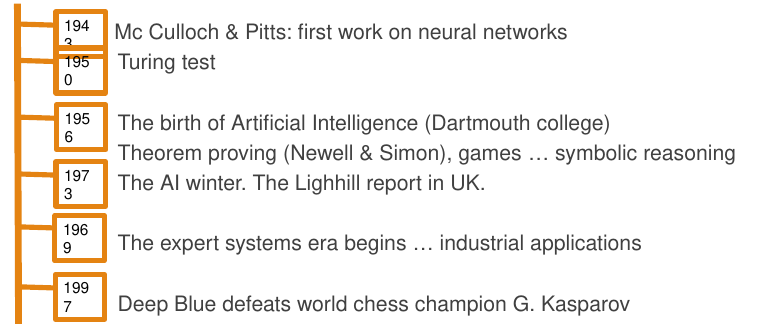
\includegraphics[width=\textwidth]{Images/timeline}
    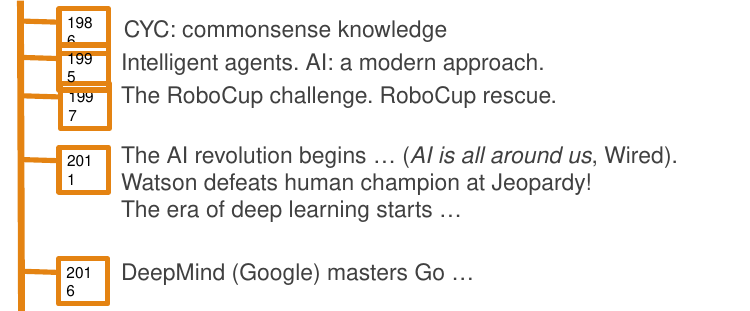
\includegraphics[width=\textwidth]{Images/timeline2}
\end{figure}
The major discover happened on $2020$ are the following:
\begin{description}
    \item [GPT3 (Generative Pre-trained Transformer): ] produced by OpenAI in May $2020$, is 
           a larger and richer language model consisting in $175$ billion machine learning parameters
           used for automatic text generation, translation, user interface synthesis
    \item [DARPA challenge (AlphaDogFights)] with simulated F-16 Air Fighters where on $18-20$ August $2020$
           there was the final Event, where AI system was against each other and the winner was a system by 
           Heron system, that was also able to defeated a human expert top gun fighter $5-0$.
\end{description}
On \cite{andrewNg} Andrew NG says that AI will transform many industries, but it’s not magic and 
almost all of AI’s recent progress is based on one type of AI, in which some input data $(A)$ is used to
quickly generate some simple response $(B)$ [$A \to B$].\newline
Also Andrew Ng says that if a typical person can do a mental task with less than one second of thought,
we can probably automate it using AI either now or in the near future.\newline
Choosing A and B creatively has already revolutionized many industries, it is poised to
revolutionize many more.

ML systems are not (yet?) able to justify in human terms their results, so for some application it is essential
the human knowledge to be able to generate explanations, infact some regulations requires the right
to an explanation in decision-making, and seek to prevent discrimination based on race, opinions,
health, sex and so on, like GPDR.\newline
ML systems learn what’s in the data, without understanding what's true or false, real or imaginary, 
fair or unfair and so it is possible to develop bad/unfair models.

The goal of building AI systems is far from being solved and is still quite challenging in its own.
Building complex AI systems requires the combination of several techniques and approaches, not only ML.\newline
One of the most challenging tasks ahead of us is integration of
perception and reasoning in AI systems.

AI fundamentals is mostly about “Slow thinking” or “Reasoning” and AI fundamentals has the role,
within the AI curriculum, of teaching you about the foundations of a discipline which is now 60 year old.\newline
We will cover different approaches, also some coming of the “Good Old-
Fashioned Artificial Intelligence” (GOFAI) or symbolic AI.

\begin{defi}
Symbolic AI is an high-level "symbolic" (human-readable) representations of problems, the 
general paradigm of searching for a solution, knowledge representation and reasoning, planning.\newline
Symbolic AI was the dominant paradigm of AI research from the mid 1950s until the late 1980s and 
central to the building of AI systems is the \emph{Physical symbol systems hypothesis}, formulated by Newell and Simon.
\end{defi}

The approach is based on the assumption that many aspects of intelligence can be achieved by the 
manipulation of symbols (the physical symbol system hypothesis):
\begin{defi}
A physical symbol system has the necessary and sufficient means for general intelligent action
\end{defi}%CITE WHO SAYS THAT
Human thinking is a kind of symbol manipulation system (a symbol system is necessary for intelligence) and 
machines can be intelligent (a symbol system is sufficient for intelligence).\newline
The hypothesis cannot be proven, we can only collect empirical evidence and observations and experiments
on human behavior in tasks requiring intelligence.

We have two different typologies of AI, that was introduced and considered:
\begin{description}
    \item [Strong AI: ] relies on the strong assumption that human intelligence can be reproduced
                        in all its aspects (general A.I.).\newline
                        It includes adaptivity, learning, consciousness and not only pre-programmed behavior.
    \item [Weak AI: ]   simulation of human-like behavior, without effective thinking/understanding and 
                        no claim that it works like human mind; it is the dominant approach today.
\end{description}
A problem of AI is that computer can't have needs, cravings or desires and Abraham Maslow's define 
a hierarchy of human needs:
\begin{enumerate}
    \item Biological needs (food, sleep, sex, ...)
    \item Safety, protection from environment
    \item Love and belonging, friendship
    \item Self esteem and respect from others
    \item Self-actualization
\end{enumerate}

    \chapter{Background}

Matrix Product 
Vector sum
Bases
Linear system resolution

Invertibility -> Definitions

Write Block Matrices !!!
DO EXERCISE ABOUT COMPUTATIONAL MATH -> Otherwise will be a problem

    \chapter{Unconstrained optimization}
In optimization problem we want to solve 
\[ f_* = \min \{ f(x) : x \in X\} \]
and things are simpler if $X = \R^n$, which is the uncontrained optimization where only $f$ counts.

We have that $\R^n$ is not bounded so Weierstrass does not apply and turns out that is 
very difficult to recognise if a global minimum $x_*$ exists.\newline
So we will start with a weaker condition, that is that $x_*$ is local minimum if it solves
\[ \min \{f(x): x \in B(x_*, \epsilon)\} \,\, \epsilon > 0 \]
A stronger notion is that we have a strict local minimum if 
$f(x_*) < f(y) \, \forall y \in B(x_*, \epsilon)$.

As can be viewed in figure \ref{img:localOptimality}, we have that in all local (global) minima
we have $f^'(x) = 0$, but also in local (global) maxima and in saddle points.
\begin{figure}
    \includegraphics[width=0.7\textwidth]{Images/localOptimality}
    \caption{Representation of local optima on Cartexian axis}
    \label{img:localOptimality}
\end{figure}
\begin{thm}
    If $f$ is differentiable we have if $x$ is a local minimum then $\Delta f(x) = 0$.
\end{thm}
\begin{proof}
    We prove by contradiction and to prove that $x$ is not a local minimum we have to exhibit
    a better points, which $\Delta f(x)$ will tell us.\newline
    We define $x(\alpha) = x - \alpha \Delta f(x)$, which is a step along the anti-gradient 
    $-\Delta f(x)$ and also $\phi(\alpha) = f(x(\alpha))$, the univariate restriction of $f$ 
    on line $-\Delta f(x)$ from $x$.\newline
    We want to prove that exists $\bar{\alpha} > 0$ such that $\phi(\bar{\alpha}) < f(x)$ and 
    we have $f:\R^n \to \R \in C^1$ in some $B(x, \delta)$.

    Using the first-order Taylor's formula, with remainder we have that
    \[ f(y) = L_x(y) + R(y - x) = <\Delta f(x), y - x> + f(x) + R(y-x) \]
    with $\lim_{h \to 0} R(h)/\norm{h} = 0$.

    We have that $R(y - x)$ is the remainder, which vanishes at least quadratically fast as 
    $y \to x$, visible as $O(\norm{y - x}^2)$.\newline
    Using Taylor we have that
    \[ \phi(\alpha) = f(x - \alpha \Delta f(x)) = f(x) + <-\alpha \Delta f(x), \Delta f(x)>
                                                       + R(-\alpha \Delta f(x)) \]
    Using the definition of $\norm{*}$ with also the property of $<*, *>$ we get
    \[ \phi(\alpha) = f(x) - \alpha \norm{\Delta f(x)}^2 + R(-\alpha \Delta f(x)) \]

    As $\alpha \to 0$ we have that 
    \[ \lim_{\alpha \to 0}R(-\alpha \Delta f(x))/\norm{\alpha \Delta f(x)} = 
       \lim_{\norm{h} \to 0} R(h) / \norm{h} = 0 \]
    which is equivalent to have 
    \[ \forall \epsilon > 0 \exists \bar{\alpha} > 0 \, R(-\alpha \Delta f(x)) / 
            \alpha \norm{\Delta f(x)} \leq \epsilon \,\, \forall 0 \leq \alpha \leq \bar{\alpha} \]
    Taken $\epsilon < \norm{\Delta f(x)}$ we get $R(-\alpha \Delta f(x)) < 
    \alpha \norm{\Delta f(x)}^2$ which imply that 
    \[ \phi(\alpha) = f(x) - \alpha \norm{\Delta f(x)}^2 + R(-\alpha \Delta f(x)) < f(x) 
           \forall \alpha < \bar{\alpha} \]
    From this fact we can prove that $x$ cannot be a local minimum.
\end{proof}
With first-order we can't recognize that we are on a stationary point, so we need to look at 
curvature of $f$, so if $f$ was quadratic we would know, since we look at eigenvalues of 
$Q = \Delta^2 f(x)$.\newline
Obvious idea consist to approximate $f$ with a quadractic function, the second-order model
\[ Q_x(y) = L_x(y) + \frac{1}{2}\transpose{(y - x)}\Delta^2 f(x)(y - x) \]
and also that $\Delta Q_x(x) = \Delta f(x)$ and also $\Delta Q_x(x) = 0$.

We have also that $\Delta^2 f(x) \succeq 0 \iff x \text{ (global) minimum of } Q_x$ and we can
also prove this following theorem
\begin{thm}
    If $f \in C^2, x$ local mimimum then we have $\Delta^2 f(x) \succeq 0$
\end{thm}
\begin{proof}
    We have the second-order Taylor's formula
    \[ f(y) = L_x(y) + \frac{1}{2}\transpose{(y-x)}\Delta^2 f(x) (y - x) + R(y - x) \]
    with $\lim_{\norm{h} \to 0} R(h) / \norm{h}^2 = 0$, so the error is $O(\norm{y-x}^3)$ and
    of course $k$-th order Taylor expansion with $k$-th order derivatives with $\Delta^k f(x)$ 
    tensor of order $k$.

    For $n$ large even $n^2$ too much and Gradient and Hessian give the best second-order model 
    of $f$ at $x$ and to prove this optimality condition we use the proof by contradiction.\newline
    We define $d$ as the direction of negative curvature and we have 
    \[ x(\alpha) = x + \alpha d \, \phi(\alpha) = f(x(\alpha)) \]
    If we have second-order Taylor formula and $\Delta f(x) = 0$, so we have $L_x(y) = f(x)$ and then
    \[ \phi(\alpha) = f(x) + \frac{1}{2}\alpha^2 \transpose{d} \Delta^2 f(x) d + R(\alpha d) \]
    which is a negative quadractic term in $\alpha$ and a possibly positive "cubic" one.

    As $\alpha (= \norm{h = \alpha d}$ since $\norm{d} = 1) \to 0$, it is clear who wins, so
    \[ \lim_{\alpha \to 0} R(\alpha d) / \alpha^2 = \lim_{\norm{h} \to 0} R(h) / \norm{h}^2 = 0 \]
    which is equivalent to have
    \[ \forall \epsilon > 0 \exists \bar{\alpha} > 0 \, R(\alpha d) \leq \epsilon \alpha^2 \,
	                                                \forall 0 \leq \alpha \leq \bar{\alpha} \]
    If we take $0 < \alpha < -\frac{1}{2}\transpose{d}\Delta^2 f(x) d$ we get 
    \[ R(\alpha d) < -\frac{1}{2}\alpha^2\transpose{d}\Delta^2 f(x) d \]
    which yields to
    \[ \phi(\alpha) = f(x) + \frac{1}{2} \alpha^2 \transpose{d} \Delta^2 f(x) d + R(\alpha d) < f(x)
	\forall 0 \leq \alpha < \bar{\alpha} \]
    In a local minimum there cannot be directions of negative curvature, so when the first derivative
    is $0$, the second-order effects prevail.
\end{proof}
The necessary condition (yet proved) is almost also sufficient, so if $f \in C^2, \Delta f(x) = 0$ and
$\Delta^2 f(x) \succ 0$ then $x$ is strict local minimum.

To find global mimima we should avoid local-non-global minima, and we have also that all stationary
points must be local mimima, so $\Delta f(x) = 0 \Rightarrow \Delta^2 f(x) \succeq 0$.\newline
The sufficient condition is that $\Delta^2 f(x) \succeq 0 \, \forall x \in \R^n$ imply 
that $f$ is a convex function.

\section{Convex sets and functions}
We define the segment joining two points $x$ and $y$ as 
\[ conv(x, y) = \{\alpha x + (1 - \alpha) y: \alpha \in [0, 1], x, y \in \R^n\} \]
We have that a set $C \subset \R^n$ is \emph{convex} if $\forall x, y \in C \, conv(x, y) \subseteq C$
and is nonconvex in case $\exists x, y \in C \, conv(x, y) \not \subseteq C$.

Every nonconvex set can be completed to a convex set using this formula
\begin{align*}
	conv(S) & = \cup \{conv(x, y): x, y \in S\} \\
	        & = \cap \{C: C \text{ is convex } \land C \supseteq S \} \\
\end{align*}
We have that the \emph{convex Hull} of $S$ is the smallest convex set containing $S$ and we have 
$C$ is convex $\iff C = conv(C)$.

An apparently more general, but in fact equivalent, definition is the following 
\[ conv(\{x_1, \dots, x_k\}) = \{x = \sum_{i=1}^k \alpha_i x_i: \sum_{i=1}^k \alpha_i = 1, 
                                                         \alpha_i \geq 0 \forall i \} \]
We have also that 
\[ \Theta^k = \{\alpha_i \in \R^k: \sum_{i=1}^k \alpha_i = 1, \alpha_i \geq 0 \, \forall i\} \]
which is the unitary simplex in $\R^k$ and also that if $C$ is convex then 
$C \supseteq conv(\{x_1, \dots, x_k\}) \forall x_1, \dots, x_k \in C$.

We have in figure \ref{img:interestingConvex} we have some example of Convex sets and also 
which are some convex sets that are also cones.
\begin{figure}
	\includegraphics[width=\textwidth]{Images/interestingConvex}
	\caption{Interesting Convex Sets and Cones}
	\label{img:interestingConvex}
\end{figure}
The operations that preserve convexity are the following:
\begin{itemize}
    \item $\{C_i\}_{i \in I}$ a possibly infinite family of convex sets imply $\cap_{i \in I} C_i$ convex.
    \item $C_1, \dots, C_k$ convex if and only if $C_1 \times \dots \times C_k$ convex.
    \item $C$ convex imply $A(C) = \{x = Ay + b: y \in C\}$ convex.
    \item $C$ convex imply $A^{-1}(C) = \{x: Ax + b \in C\}$ convex.
    \item $C_1$ and $C_2$ convex, $\alpha_1, \alpha_2 \in \R$ imply that is convex 
	    \[ \alpha_1C_1 + \alpha_2C_2 = \{x = \alpha_1x_1 + \alpha_2x_2: x_1 \in C_1, x_2 \in C_2\} \]
    \item $C \subseteq \R^n = \R^{n_1} \times \R^{n_2}$ convex imply that 
	    \[ C(y) = \{x \in \R^{n_1}: (x, y) \in C\} \text{ is convex (slice) } \]
	    \[ C^1 = \{x \in \R^{n_1}: \exists y (x, y) \in C\} \text{ is convex (shadow)} \]
    \item $C$ convex imply that $int(C)$ and $cl(C)$ is convex.
\end{itemize}
We have that $f$ convex is equivalent to $epi(f)$ convex, so also equivalently we have 
\[ \forall x, y \in dom(f), \alpha \in [0, 1] \, \alpha f(x) + (1 - \alpha)f(y) \geq f(\alpha x + (1 - \alpha)y) \]
Equivalently we have that $\forall x^1, \dots, x^k, \alpha \in \Theta^j$
\[ f(\sum_{i=1}^k \alpha_i x^i) \leq \sum_{i=1}^k \alpha_i f(x^i) \]
If $f$ is convex then $S(f, v)$ is convex for all $v \in \R$ and also that $f$ is concave if $-f$ is convex.

\begin{defi}[Strictly convex]
    We have that $f$ is strictly convex if results
    \[ \alpha f(x) + (1 - \alpha)f(y) > f(\alpha x + (1 - \alpha)y) \]
\end{defi}
\begin{defi}[Strongly convex]
    We have $f$ strongly convex modulus $\tau > 0$ in case results $f(x) - \frac{\tau}{2}\norm{x}^2$ which is 
    equivalent to 
    \[ \alpha f(x) + (1 - \alpha)f(y) \geq f(\alpha x + (1-\alpha)y) + \frac{\tau}{2}\alpha(1-\alpha)\norm{y-x}^2 \]
\end{defi}
In figure \ref{img:convexFunctions} we have some example of convex functions, and also 
in figure \ref{img:convexFunctionalOp} is possible to note functional operations that preserve convexity.

If $f$ convex we have that $\Delta f$ exists almost everywhere and $f \in C^1$ convex on $C$ convex if and only if
\[ f(y) \geq f(x) + <\Delta f(x), y - x> \forall x,y \in C \]
We have $f$ strictly convex with $>$ and $f$ strongly convex if the inequality of convex holds
also if we add a term $\frac{\tau}{2} \norm{y-x}^2$.

We have from first-order model that 
\[ L_x(y) = f(x) + <\Delta f(x), y - x> \leq f(y) \]
We have also that $\Delta f(x) = 0 \Rightarrow f(y) \geq f(x) \forall y \in \R^n$ and if $f \in C^1$ convex we 
have $x$ is a stationary point if and only if $x$ is a global minimum.\newline
In case $f \in C^2$ we have $f$ convex on $S$ if and only if $\Delta^2 f(x) \succeq 0 \forall x \in S$ and 
$f \in C^2$ with $\Delta^2 f \succ 0$ is the best case for optimization.


    \printbibliography
\end{document}
